%% sample template file for a BSc Thesis
%% The default is the norsk version with two sided setup:
\documentclass[%
    norsk,  % comment for english version
%    oneside % uncomment for onesided layout
]{USN-BSc}

% --- Bibliography setup ---
%%% default is the "numberic" style
\usepackage[style=numeric, sorting=none]{biblatex}
%%% If you want to use "author-year" style
%%% where `\cite{Foo2011}` generates "Foo et al. (2011)"
%%% and   `\parentcite{Foo2011}` generates "(Foo et al. 2011)"
%%% then comment the line above and use
%\usepackage[style=authoryear]{biblatex}
%%% or
%%% if you want to use "alphabetic" style then use
%%% where `cite[Foo2011]` generates "[Foo11]"
%%% then comment the line above and use
%\usepackage[style=alphabetic]{biblatex}
%%% instead.
%% load the bib file:
\addbibresource{thesis.bib}

\usepackage{lipsum} % just for providing fill text used in this template

% --- general setup ---
%% Please fill in the following parameters:
\newcommand{\mytitle}{%
%% title:
<prosjektets tittel>
}

\newcommand{\mysubtitle}{%
%% subject code:
<emnekode og emnenavn>
}

\newcommand{\myauthor}{%
%% group code:
<gruppekode>
}

\newcommand{\supervisor}{%
%% supervisor:
<veildeder>
}

\newcommand{\examiner}{%
%% examiner:
<sensor>
}


\begin{document}

% --- title page setup ---
\USNtitlepage%
%% Please provide the following information:
%% #1 semster:
{1}
%% #2 optional figure (set to {} if not wanted)
{~%\vfill
   
\includegraphics[draft,width=\textwidth]{HSN_logo_en}}
%% #3 date
{\today}  % leave this empty to deactivate display
%% #4 group members
{%
<første deltaker, NB! Ingen signatur her>\\
<andre deltaker, NB! Ingen signatur her>\\
<tredje deltaker, NB! Ingen signatur her>\\
<fjerde deltaker, NB! Ingen signatur her>\\
<femte deltaker, NB! Ingen signatur her>\\
<sjette deltaker, NB! Ingen signatur her>
}
%% #5 confidential?:
{yes} % anything other then {yes} means open to public
% #6 Project partner:
{<Prosjektpartner>}
%% #7 Norwegian Summary:
{%
\lipsum[6-7]
}
%% #8 English Summary:
{%
\lipsum[6-7]
}

%% The chapter name for preface is set depending on language
\chapter*{\USNpreface}
\label{sec:preface}
\addcontentsline{toc}{chapter}{\USNpreface}
\lipsum[1-3]

\tableofcontents
\addcontentsline{toc}{chapter}{\contentsname}

\listoffigures % out-comment if unwanted
\addcontentsline{toc}{section}{\listfigurename}

\listoftables  % out-comment if unwanted
\addcontentsline{toc}{section}{\listtablename}

\chapter*{Nomenclature}
\label{sec:nomenclature}

\begin{longtable}{ll}
  \textbf{Symbol} & \textbf{Explanation}\endhead\\
  A/D	& Analogue-Digital-Converter \\
  CMR	& Common Mode Rejection \\
  foo	& Foo \\
  bar 	& Bar
\end{longtable}


%\mainmatter
%\part{Overview}  %% DO NOT USE \part FOR MONOGRAPHY
%\label{part:overview}
\chapter{Introduction}
\label{ch:intro}


\lipsum[4]
\begin{figure}[!ht]
  \centering
  
\includegraphics[width=0.8\textwidth]{HSN_logo}
  \caption{Norwegian (bokmål) variant of the HSN logo}
  \label{fig:hsn-logo}
\end{figure}
\lipsum[4]
\begin{figure}[!ht]
  \centering
  
\includegraphics[width=0.8\textwidth]{HSN_logo_en}
  \caption{English variant of the HSN logo.}
  \label{fig:hsn-logo-en}
\end{figure}
\lipsum



\section{Background}
\label{sec:back}
\lipsum[4]
\begin{equation}
  e = m c^2
\end{equation}
\lipsum

\chapter{Theory}
\label{ch:theory}

\section{Maxwell's Equations}
\label{sec:theory}
\indent The differential forms of Maxwell's equations as found by Heaviside, while completely valid, are now considered somewhat archaic, and have been replaced by the more useful (equivalent) integral forms. Each law is named according to the person(s) who originally discovered the connections represented by the equation. Here are the four equations:
\begin{eqnarray}
  \text{Gauss' law for electricity:}& \displaystyle \oint{\vec{E}\cdot\mathrm{d}\vec{A}}&=\frac{Q_{enc}}{\epsilon_0}\\
  \text{Gauss' law for magnetism:}& \displaystyle \oint{\vec{B}\cdot\mathrm{d}\vec{A}}&=0\\
  \text{Faraday's law:}& \displaystyle\oint{\vec{E}\cdot\mathrm{d}\vec{s}}&=-\frac{\emph{d}\phi_b}{\mathrm{d}t}\\
  \text{Ampere-Maxwell law:}& \displaystyle\oint{\vec{B}\cdot\mathrm{d}\vec{s}}&=\mu_0\epsilon_0\frac{\emph{d}\phi_e}{\mathrm{d}t}+\mu_0 i_{enc}
\end{eqnarray}
Note: $\oint$ is used to specify a closed loop integral, also known as a line integral. It simply means that in the calculations, we must go all the way around the loop; we can't stop part way through or the equations won't be valid.

\section{Mathematical model}
\label{sec:mathmodel}
\lipsum[8]
\begin{table}[!ht]
  \caption{The different number systems}
  \centering
  \begin{tabular}{|r|l|}
    \hline
    7C0 & hexadecimal \\
    3700 & octal \\ \cline{2-2}
    11111000000 & binary \\
    \hline \hline
    1984 & decimal \\
    \hline
  \end{tabular}
\end{table}

\lipsum[4]

\begin{table}[!ht]
 \caption{The weather forecast}
  \centering
   \begin{tabular}{ | l | l | l | p{5cm} |}
    \hline
    Day & Min Temp & Max Temp & Summary \\ \hline
    Monday & 11C & 22C & A clear day with lots of sunshine.
    However, the strong breeze will bring down the temperatures. \\ \hline
    Tuesday & 9C & 19C & Cloudy with rain, across many northern regions. Clear spells
    across most of Scotland and Northern Ireland,
    but rain reaching the far northwest. \\ \hline
    Wednesday & 10C & 21C & Rain will still linger for the morning.
    Conditions will improve by early afternoon and continue
    throughout the evening. \\
    \hline
    \end{tabular}
\end{table}


% A dummy command that causes all bibliographyentries to be displayed
% even though there were not cited in the document. Used for demonstration
% purposes only in this template file.
~\nocite{*}

\cleardoublepage

% The bibliography should be displayed here...
\printbibliography[heading=bibintoc]
% You rather like to call the bibliography "References"? Then use this instead:
%\printbibliography[heading=bibintoc, title={References}]


\appendix
\renewcommand{\appendixname}{Paper} %% So we get 'Paper X' displayed instead

%\part{Published and Submitted Papers}  %% DO NOT USE \part FOR MONOGRAPH
%\label{part:papers}


\chapter[Short Title of Paper A]{Title of Paper A (probably very long and therefore not good to have in the header)}
\label{paper-a}

\paragraph{Note}
Since some papers tend to have a rather long title it is good to provide the optional short title which then will be displayed in the table of contents and header instead of the long original title.
On the openening page of the chapter the orginal \emph{long} title will be displayed.\bigskip

\emph{Short descriptive text of paper follows here.}\bigskip

The paper itself needs to be included in the published form as PDF on the next pages.
This can be done using the \texttt{pdfpages} package by adding the command:

\begin{verbatim}
\includepdf{pages=-,openright}{Filename}
\end{verbatim}

You can ommit the \texttt{.pdf} when specifying the \texttt{Filename}. Also you should include always include the option \texttt{openright} since it would look strange to have the paper starting at the back of the cover page.

There are more options like only adding specific pages:
\begin{verbatim}
\includepdf{pages=2-6,openright}{Filename.pdf}
\end{verbatim}

For more options see Appendix~\ref{paper-b} where the most important pages of the \texttt{pdfpages} manual were inlcuded using \texttt{pdfpages}.


%%% Command to include a PDF file directly including all pages:


\chapter[Short Title of Paper B]{Title of Paper B}
\label{paper-b}
Short descriptive text of paper follows here.

Here we included the first five pages of the \texttt{pdfpages} manual itself.

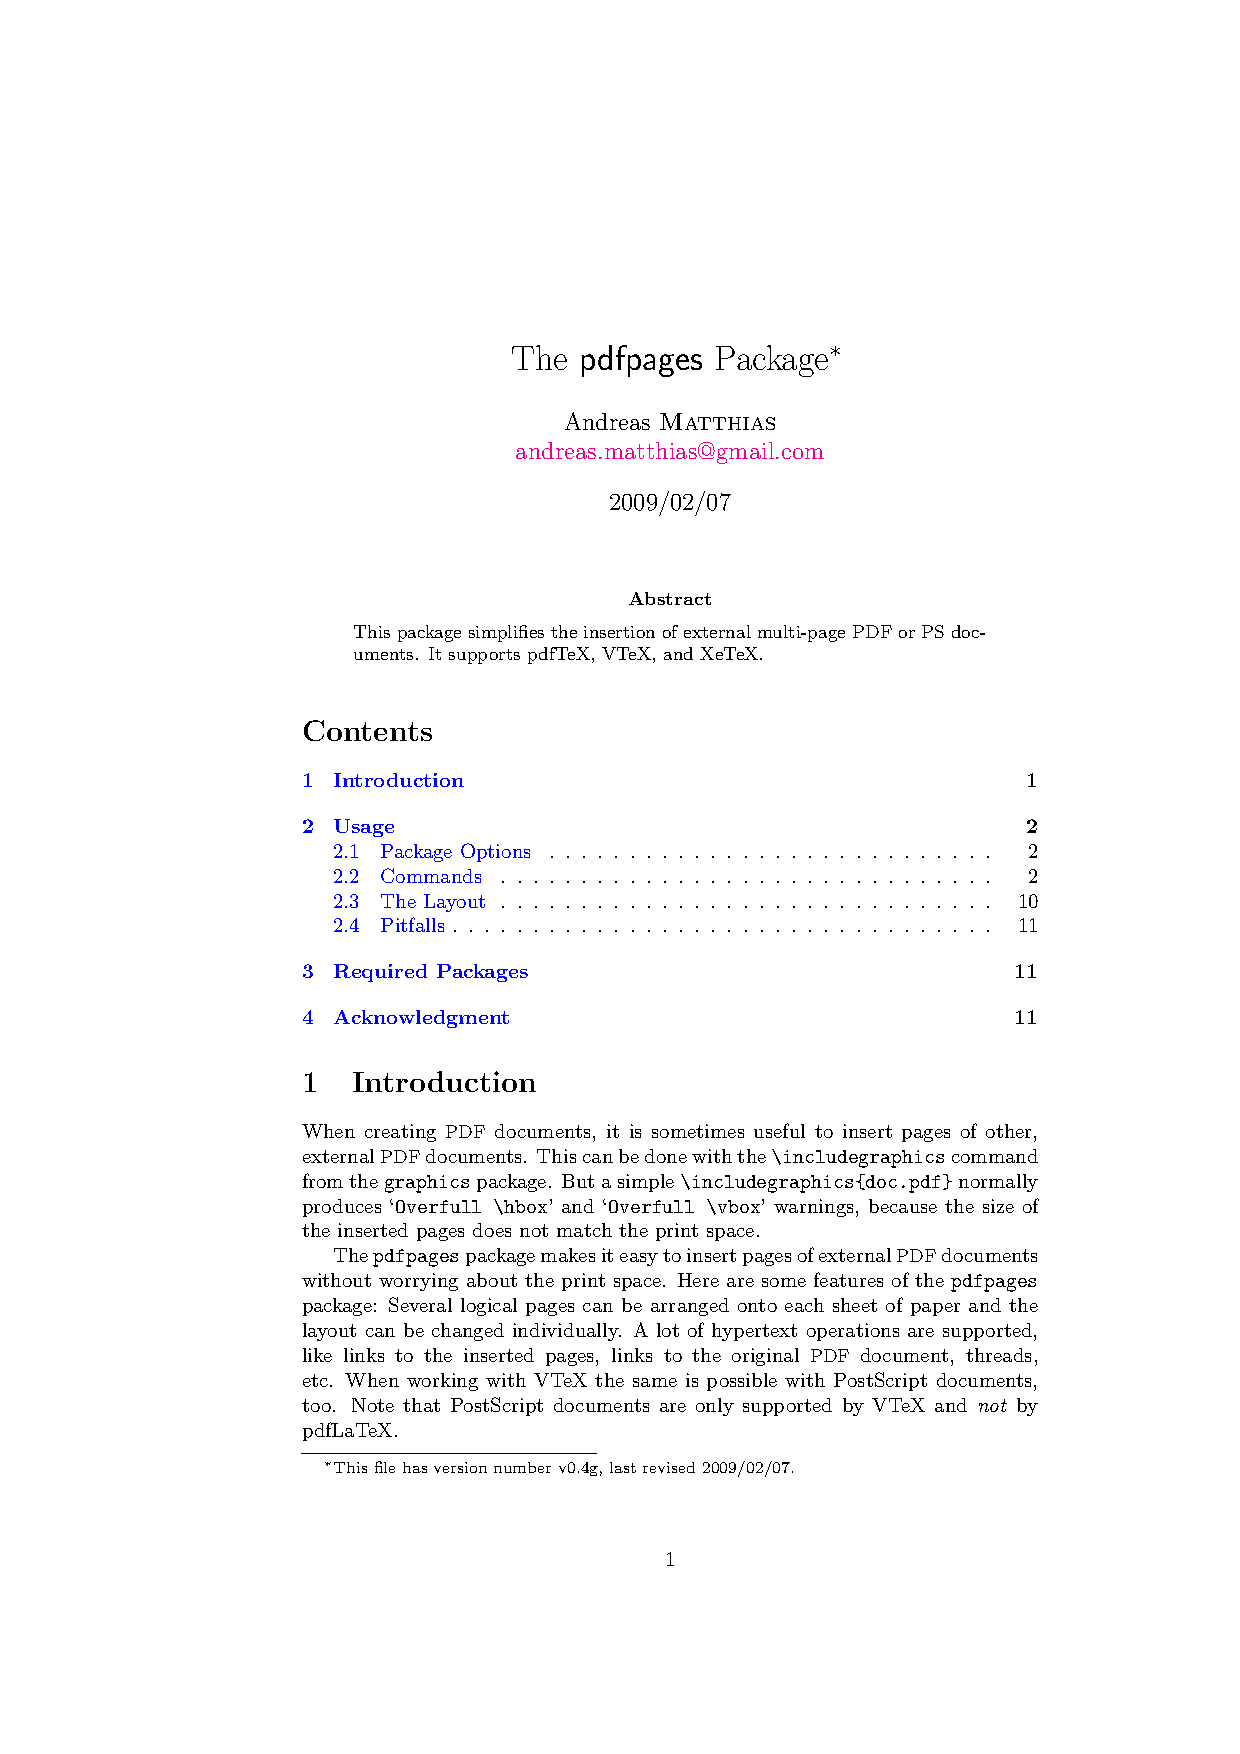
\includepdf[pages=1-5,openright]{fig/pdfpages}

\end{document}

%%% Local Variables:
%%% mode: latex
%%% TeX-master: t
%%% End:
